%%%%%%%%%%%%%%%%%%%%%%%%%%%%%%%%%%%%%%%%%%%%%%%%%%%%%%%%%%%%%%%%%%%%%%%%%%%%%%%%
% Template for USENIX papers.
%
% History:
%
% - TEMPLATE for Usenix papers, specifically to meet requirements of
%   USENIX '05. originally a template for producing IEEE-format
%   articles using LaTeX. written by Matthew Ward, CS Department,
%   Worcester Polytechnic Institute. adapted by David Beazley for his
%   excellent SWIG paper in Proceedings, Tcl 96. turned into a
%   smartass generic template by De Clarke, with thanks to both the
%   above pioneers. Use at your own risk. Complaints to /dev/null.
%   Make it two column with no page numbering, default is 10 point.
%
% - Munged by Fred Douglis <douglis@research.att.com> 10/97 to
%   separate the .sty file from the LaTeX source template, so that
%   people can more easily include the .sty file into an existing
%   document. Also changed to more closely follow the style guidelines
%   as represented by the Word sample file.
%
% - Note that since 2010, USENIX does not require endnotes. If you
%   want foot of page notes, don't include the endnotes package in the
%   usepackage command, below.
% - This version uses the latex2e styles, not the very ancient 2.09
%   stuff.
%
% - Updated July 2018: Text block size changed from 6.5" to 7"
%
% - Updated Dec 2018 for ATC'19:
%
%   * Revised text to pass HotCRP's auto-formatting check, with
%     hotcrp.settings.submission_form.body_font_size=10pt, and
%     hotcrp.settings.submission_form.line_height=12pt
%
%   * Switched from \endnote-s to \footnote-s to match Usenix's policy.
%
%   * \section* => \begin{abstract} ... \end{abstract}
%
%   * Make template self-contained in terms of bibtex entires, to allow
%     this file to be compiled. (And changing refs style to 'plain'.)
%
%   * Make template self-contained in terms of figures, to
%     allow this file to be compiled. 
%
%   * Added packages for hyperref, embedding fonts, and improving
%     appearance.
%   
%   * Removed outdated text.
%
%%%%%%%%%%%%%%%%%%%%%%%%%%%%%%%%%%%%%%%%%%%%%%%%%%%%%%%%%%%%%%%%%%%%%%%%%%%%%%%%

\documentclass[letterpaper,twocolumn,10pt]{article}
\usepackage{usenix-2020-09}

% to be able to draw some self-contained figs
\usepackage{tikz}
\usepackage{amsmath}
\usepackage{makecell}
\usetikzlibrary{datavisualization}

\renewcommand\theadalign{bc}
\renewcommand\theadfont{\bfseries}

% inlined bib file
\usepackage{filecontents}


%-------------------------------------------------------------------------------
\begin{document}
%-------------------------------------------------------------------------------


% make title bold and 14 pt font (Latex default is non-bold, 16 pt)
\title{\Large \bf Enhancing Quanto:\\Pruning Techniques for Improved Circuit Identity Generation in Quantum Optimization}

%for single author (just remove % characters)
\author{
{\rm Max von Storch}\\
Technical University of Munich
\and
{\rm Johannes Schielein}\\
Technical University of Munich
% copy the following lines to add more authors
% \and
% {\rm Name}\\
%Name Institution
} % end author

\maketitle

%-------------------------------------------------------------------------------
\begin{abstract}
%-------------------------------------------------------------------------------
This report summarizes Quanto \cite{2021quanto}, a quantum circuit optimizer that uses automated circuit identity generation. We propose enhancements to Quanto by focusing on pruning the search space of possible circuits, aiming to improve computational efficiency and scalability, particularly for larger circuits.  
\end{abstract}


%-------------------------------------------------------------------------------
\section{Paper Summary}
%-------------------------------------------------------------------------------

\subsection{Context and Importance}

Quantum compilers are used to optimize circuits in an effort to reduce execution time, the noise that naturally arises in quantum computations, or both. Generally, the larger the circuit depth, the noisier the computation, leading to more errors in the results. As quantum programs must be executed many times to obtain an accurate picture of their results, reducing the depth of a quantum circuit not only makes a quantum program faster but also reduces the potential for noise and decreases the number of program evaluations required.
\\\\
Existing quantum compilers focus on mapping logical quantum circuits to quantum devices and their native quantum gates. This involves translating source gates to target gates and adapting the circuit to hardware constraints like qubit connectivity. Typically, only simple circuit identities are used during this process, which overlooks the potential for more complex optimizations.
\\\\
Compilers developed by hardware vendors, such as IBM \cite{2017qiskit} and Google \cite{2018cirq}, primarily address the translation and hardware adaptation aspects but focus less on optimizing the logical circuit by finding comprehensive circuit identities. While circuit identities have been manually identified and automatically generated for single-qubit gates by applying a limited number of rules, no current system automatically finds identities for complete gate sets or optimizes quantum circuits based on these identities.

\begin{figure}
  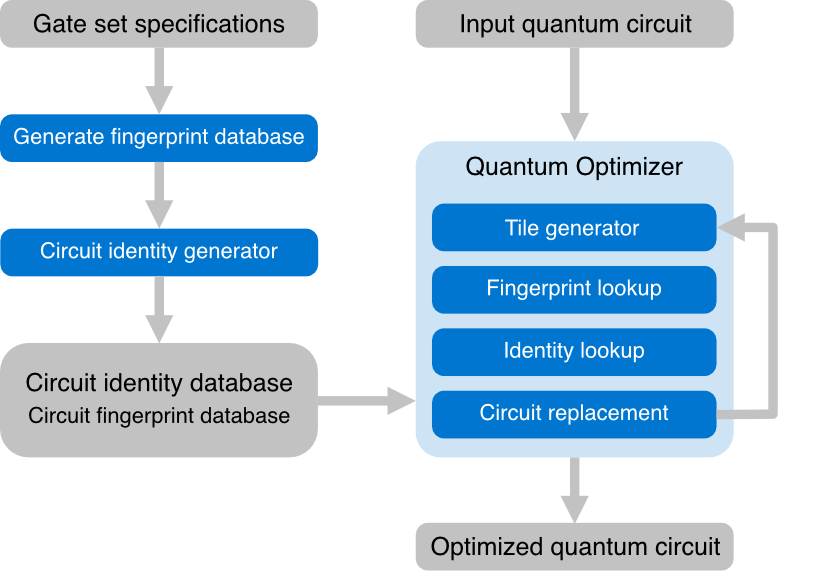
\includegraphics[width=0.7\columnwidth]{assets/quanto_system.png}
  \caption{Quanto system design}
  \label{fig:quanto_system}
\end{figure}
\subsection{Contributions and Methodology}

Quanto automatically generates circuit identities for full gate sets and operates trough two main phases: \ref{gen} Identity generation and \ref{opt} circuit optimization (Fig. \ref{fig:quanto_system}).

\subsubsection{Circuit Identity Generator}
\label{gen}
\textbf{Step 1: Represent the quantum circuit as a grid.}
The algorithm starts by representing a quantum circuit as a grid with a depth $d$ and number of qubits $n$. If no gate is present at a particular position, the identity gate is placed there (Fig. \ref{fig:example_1}).
\\\\
\textbf{Step 2: Generation of all possible circuits for $d = 1$.}
If the gate set contains two-qubit gates, these gates are split into the qubits they operate on ($CX$ gate is split into $CXC$ and $CXT$ as in Fig. \ref{fig:example_1}).
\\\\
\textbf{Step 3: Generation of all possible circuits for $d > 1$.}
All subsequent circuits are generated by iteratively appending circuits of depth one ($d=1$) to each previously generated circuit. This process effectively generates the "cross-product" of circuits with the current depth and circuits of depth one.
\\\\
\begin{figure}
  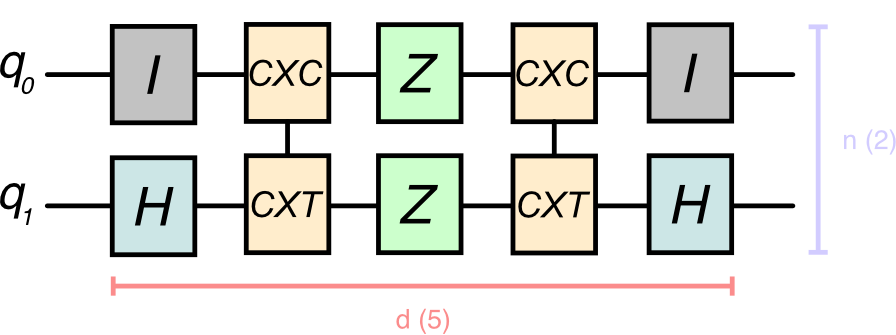
\includegraphics[width=0.8\columnwidth]{assets/grid_example_2.png}
  \caption{Example grid with identity gate substitution}
  \label{fig:example_1}
\end{figure}
\textbf{Step 4: Calculation of unitary matrices and hash values.}
For each generated circuit, the algorithm calculates the unitary matrix. To avoid expensive computations repeatedly, it computes a hash value (fingerprint) for each circuit based on its unitary matrix.
\\\\
\textbf{Step 6: Create fingerprint database.}
The fingerprints are stored in a hash table, with the circuit structure as the key and the fingerprint as the value (Table \ref{tab:databases}). This enables quick look-up of a circuit’s fingerprint during the optimization phase without recalculating the unitary matrix.

\begin{table}[h!]
  \begin{minipage}{0.4\linewidth}
    \centering
    {\renewcommand{\arraystretch}{1}%
    \begin{tabular}{|c | c|}
      \hline
      \thead{Key} & \thead{Value} \\
      \hline
      $[[H, X], [X, X]]$ & $x7ff\ldots$ \\
      \hline
    \end{tabular}}
  \end{minipage}\hfill
  \begin{minipage}{0.7\linewidth}
    \centering
    {\renewcommand{\arraystretch}{1}%
    \begin{tabular}{ |c | c | }
      \hline
      \thead{Key} & \thead{Value} \\
      \hline
       $x7ff…$ & \makecell{$[[X, X], [X, X]]$ \\
      $[[H, H], [H, H]]$}
      \\
      \hline
      \end{tabular}}
  \end{minipage}
  \caption{\label{tab:databases} Left: fingerprint DB. Right: identity DB}
\end{table}


\textbf{Step 7: Create identity database.}
Circuits with identical fingerprints are stored together, forming equivalence classes of circuits (Table \ref{tab:databases}). Each entry in this hash table represents a set of circuits that perform the same quantum operation.

\subsubsection{Circuit Optimizer}
\label{opt}
\textbf{Step 1: Generate tiles.}
The circuit is divided into sub-circuits, referred to as tiles. Tiles have uniform dimensions, with the tile width $j$ representing the maximum depth $d$ of the circuit identities, and the tile length $i$ representing the maximum number of qubits $n$ (blue boxes in Fig. \ref{fig:quanto_tile}). The number of possible $i \times j$ tiles for an $n \times d$ circuit is $(n-i+1) \cdot (d-j+1)$.
\\\\
\textbf{Step 2: Check tile validity.}
A tile is invalid and therefore discarded if it contains a two-qubit gate that is not placed at the boundaries of the tile and is cut off by the tile.
\begin{figure}
  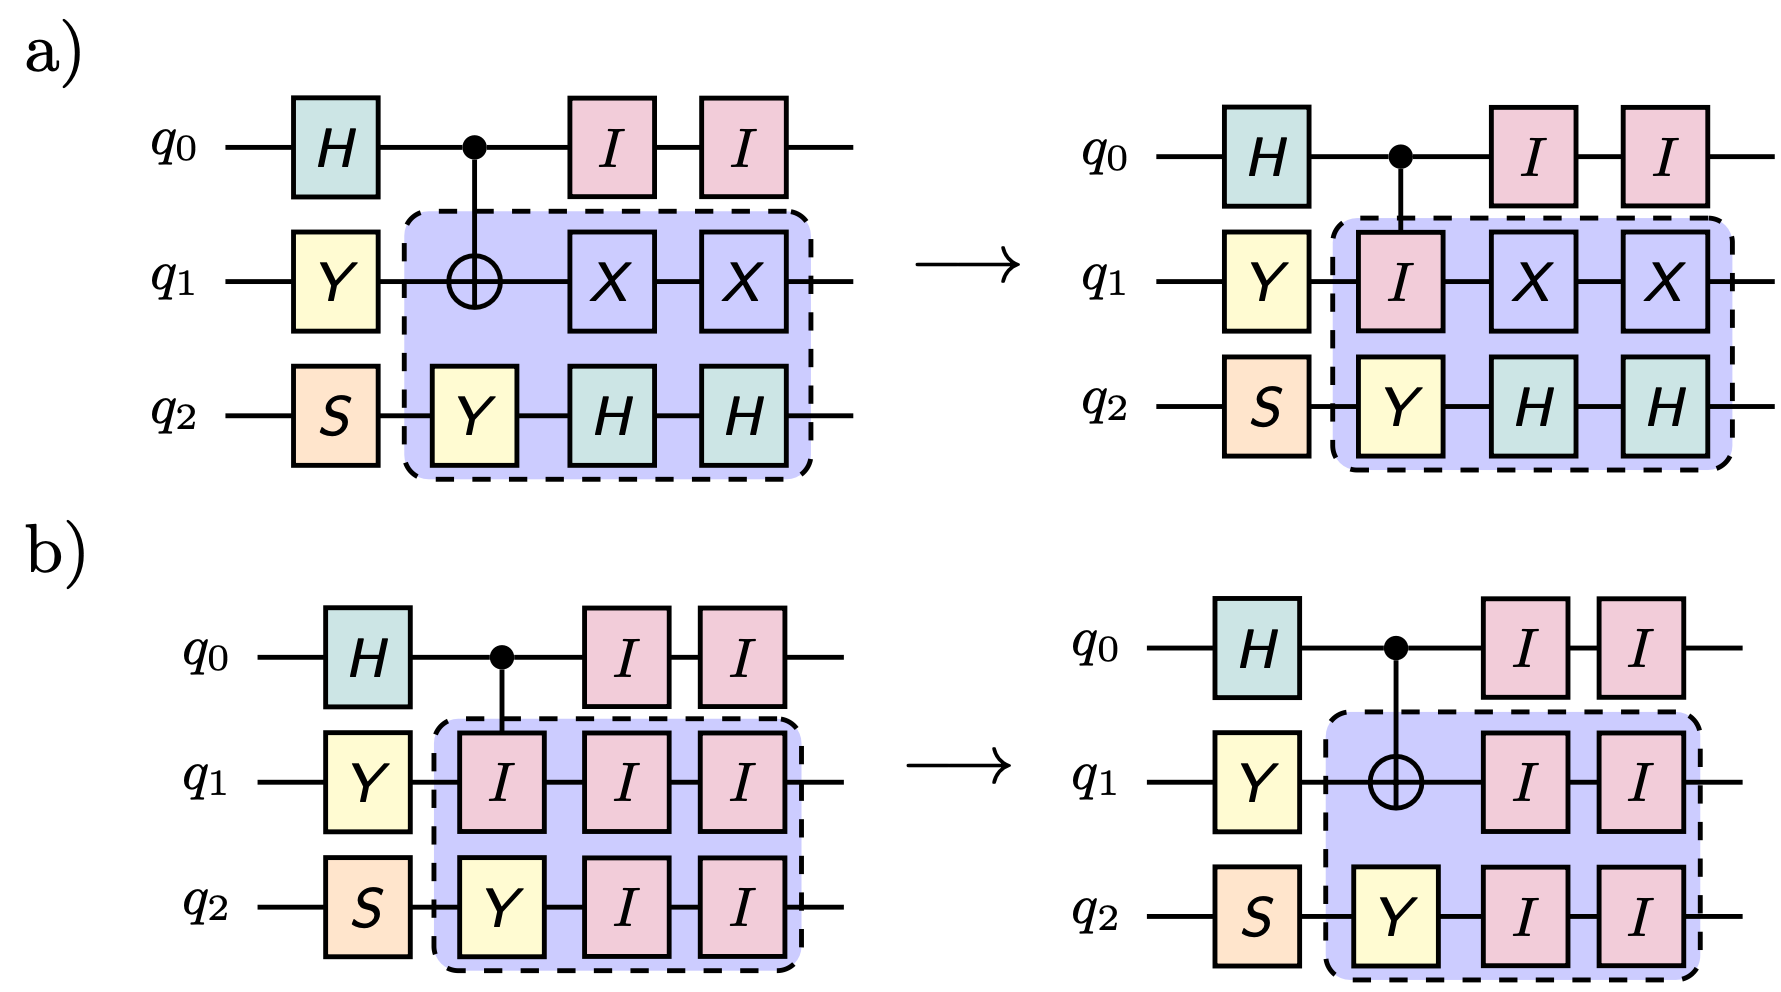
\includegraphics[width=1\columnwidth]{assets/quanto_tile2.png}
  \caption{Tile with $i=2$ and $j=3$}
  \label{fig:quanto_tile}
\end{figure}
\\\\
\textbf{Step 3: Tile lookup.}
If a tile contains a two-qubit gate, that has been cut off only at the boundaries of the tile, the cut off gate has to be replaced by an Identity gate, so that there will be a match in the circuit identity database ( a) in Fig. \ref{fig:quanto_tile}). Now the fingerprint is retrieved from the fingerprint database, without having to calculate the unitary matrix. 
\\\\
\textbf{Step 4: Apply substitution.}
For each tile, the corresponding circuit identities are iterated and evaluated by the customizable cost function (Quanto paper: depth $d$).
\\
\textbf{Step 5: Apply substitution to the circuit.}
The optimizer applies the substitution to the quantum circuit ( b) in Fig. \ref{fig:quanto_tile}). If a $CX$ gate was replaced by an identity gate in the tile, the identity gate in the actual circuit must be replaced by a $CX$ gate during the substitution. 
\\\\
\textbf{Step 6: Repeat process.}
Repeat steps 1-6 for a fixed number of times.

\subsection{Evaluation}
\subsubsection{Generation of novel identities}
Quanto is capable of automatically discovering identities known from previous work and generating novel identities for full gate sets, especially for two-qubit gates. This capability is particularly useful for quantum hardware with non-standard native gate sets.
\subsubsection{Challenge of scalability}
One of the main challenges faced by Quanto is scalability. The space of potential circuit identities scales quickly with $n$ and $d$ as described in the formula below (Symbols in Fig. \ref{tab:scaling}). This is because Quanto generates all possible identites, most of which are suboptimal.

\begin{table}
  \centering
  {\renewcommand{\arraystretch}{1}%
  \begin{tabular}{ | c | l | }
    \hline
    \thead{Symbol} & \thead{Definition} \\
    \hline
    $S$ & total number of possible circuits \\
    \hline
    $S_{l}$ & number of possible circuits per depth \\
    \hline
    $g$ & number of single-qubit gates \\
    \hline
    $t$ & number of two-qubit gates \\
    \hline
  \end{tabular}}
  \caption{\label{tab:scaling}Symbols for scaling formula}
\end{table}

\begin{equation}
     S_{l} =\sum_{r=0}^{\lfloor n/2 \rfloor}\frac{n!}{r! (n-2r)!} g^{n-2r} t^r
\end{equation}

\begin{equation}
    S = S_{l}^{d}
\end{equation}

%-------------------------------------------------------------------------------
\section{Research proposal: Pruning Methods}
%------------------------------------------------------------------------------
\subsection{Motivation}
As stated in the Quanto Paper, the exponential growth of the number of possible circuits with increasing numbers of qubits $n$ and circuit depth $d$ represents a significant limitation in the optimization of larger quantum circuits. The original method introduced tiling as a workaround, which substantially enhances the optimization level for larger circuits. However, it still falls short in delivering the same quality and speed that a database of larger circuits could achieve.
\\\\
Moreover, the current database algorithm, as proposed in the Quanto paper, stores all possible circuits, including non-optimal ones. This redundancy slows down the optimization process, as searching for minimal identities within a bloated database is computationally expensive. Pruning the search space of possible quantum circuits is thus crucial for enhancing the optimizer's performance and is worth investigating.

\subsection{Implications and Limitations}
A notable structural change in the optimizer is the elimination of the dictionary that maps circuits to their fingerprints. Due to pruning, the database generator no longer iterates over all circuits, preventing the mapping of circuits to fingerprints. Creating this dictionary in an additional step would allow grouping circuits based on their equivalence without significant computational expense, rendering pruning ineffective.
\\\\
Our research focused on optimizing the circuit depth, as it was the primary goal of the Quanto optimizer. Further investigation is necessary to determine if our approach is applicable to other cost functions.

\subsection{Notations and Definitions}
Before discussing the pruning technique, we define key terms and notations used in this section. The notation for the gate set $gs$, depth $d$, and qubit number $n$ follows the Quanto paper. The cost function for a circuit $c$ is denoted by $h(c)$.

\begin{description}
	\item[Optimal]: A quantum circuit is called optimal, if there exists no equivalent circuit (for a specified gate set) with lower cost
	
	\item[Column circuit]: A circuit with maximum depth of one
\end{description}

For concatenating two circuits $a$ and $b$ with the same number of qubits, we write $a||b$, with gates appended \textit{qubit-wise}.


% -----------------------------------------------------------------------------------
\subsection{Challenges}
Pruning the search space involves discarding certain circuits, necessitating careful selection to ensure all optimal circuits are included. Pruning adds computational overhead; thus, it is essential to balance cutting non-essential circuits and retaining enough possibilities to ensure comprehensive coverage.

\subsection{Pruning Approach}
Our research into pruning techniques began with an analysis of the Quanto database, revealing many non-optimal or redundant solutions, such as circuits with concatenated \texttt{X} gates or columns of identity gates. These non-optimal circuits are often part of larger structures and can be replaced by optimal equivalents to improve the overall circuit cost.
\\\\
Appending column circuits to a non-optimal circuit cannot yield an optimal one, as the suboptimal parts can be replaced with optimal identities (Fig. \ref{fig:approach1}). Therefore, such circuits do not need consideration in future iterations.
\\\\
However, optimal interim results may not always produce optimal end results (Fig. \ref{fig:approach2}). For instance, a minimally costly circuit ending with a column of \texttt{H} gates can become suboptimal when appended with another column of \texttt{H} gates, as they cancel each other out.
\\\\
In each iteration, new circuits can be generated, and those with higher costs than existing entries in the database can be discarded, reducing the number of circuits to consider in subsequent iterations and limiting database entries to the most optimal ones.

\begin{figure}
	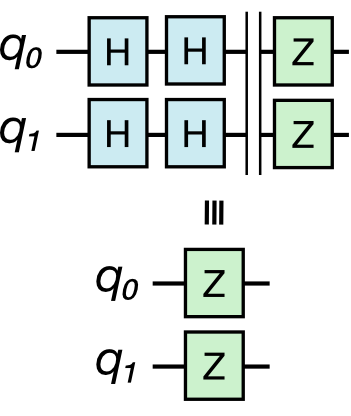
\includegraphics[width=0.8\columnwidth]{assets/approach.png}
	\caption{a can be replaced since its not optimal; c is equivalent to a$||$b}
	\label{fig:approach1}
\end{figure}

\begin{figure}
	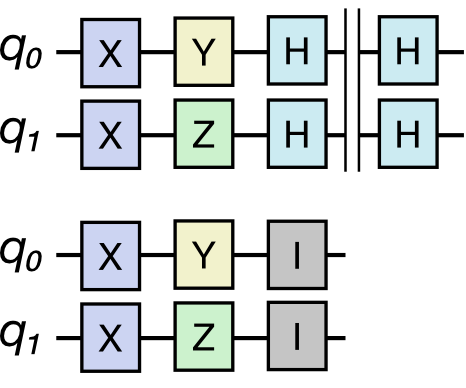
\includegraphics[width=0.8\columnwidth]{assets/approach-2.png}
	\caption{a and b are optimal but a||b is not; see c as optimal solution}
	\label{fig:approach2}
\end{figure}

\subsubsection{Proposed Algorithm}

The following pseudo-code segment demonstrates an algorithm for generating the identity database using the described pruning technique:

\begin{verbatim}
function generateDatabase(n,d,gs){
	db = dict() 	# init database
	ws = dict() 	# init Working-Set
	ws[1] = generateColumns(n,gs)
	
	for i in range(2,d) {
		for c in ws[i-1] {
			for r in ws[1] {
				c'=c||r
				if c' not in db {
					db[fingerprint(c')] = c'
					ws[i].add(c')
					continue
				}
				if isOptimal(c', db) {
					m = db[fingerprint(c')]
					db[fingerprint(c')] = c'	
					ws[i].add(c')
					ws[i].remove(m)
				}
	}}} 	# End for loops
} 	# End function
\end{verbatim}

The algorithm starts by initializing the database and a \textbf{working set} dictionary. It generates all possible column circuits for $n$ qubits and a specified gate set $gs$ using the \texttt{generateColumns(n,gs)} function.
\\\\
Next, the algorithm iterates over depth levels, starting from a depth of two up to the maximum depth 
$d$. For each iteration, it takes each element from the previous round's working set and appends every column circuit to it. Each newly generated circuit is checked to see if there is an equivalent circuit already in the database.
\\\\
If the circuit is entirely new, it is added to the current working set and the database. If an equivalent circuit exists, the algorithm checks whether the new circuit has a lower cost than the existing one. If so, the older circuit is replaced by the newly generated one in both the database and, if applicable, the current working set.
\\\\
If an optimal solution is already present, the new solution is not added to the current working set, ensuring that it will not be used in future rounds. This approach ensures that only optimal circuits are retained in subsequent iterations, effectively reducing the search space and maintaining a lean, efficient database.
\\\\
The \texttt{isOptimal(c,db)} method evaluates whether a circuit $c$ is optimal with respect to the current database $db$ and returns a boolean value accordingly.
\\\\
By following this definition, every element in the working set and the database remains optimal. For every existing circuit with $n$ qubits and depth $d$, there exists at least one equivalent circuit in the pruned database, ensuring comprehensive coverage of optimal solutions while maintaining computational efficiency.

% It follows from the definition of the algorithm that every element in $ws[i]\space\forall i$ is optimal. The same holds for the database entries.

% For every existing circuit with $n$ Qubits and depth $d$ there exists at lease an equivalent circuit in the pruned database. To show that we assume that there exists a circuit $a\Vert b$ of depth $j$ with $a\not\in ws[j-1]$. Then because of the definition of the algorithm we know that there must already exist an equivalent circuit in our database $a'$. From that it follows that $a'\Vert b\equiv a\Vert b$. Either $a'\Vert b$ is optimal and therefore in the database or there already exists an equivalent optimal circuit $c$ with $c\equiv a\Vert b$

\subsubsection{Evaluation}
The extent of reduction achieved by the proposed algorithm depends on several factors, including the circuit depth, the number of qubits, and the gate set used. Quantifying these savings can be complex. However, it is clear that removing even a single non-optimal circuit in an iteration results in a significant reduction in the number of circuits considered in subsequent iterations. Specifically, for $S_l$ column circuits, the removal of one circuit in the $k$-th iteration leads to $S_l^{d-k}$ fewer circuits being processed by the algorithm (Table \ref{tab:scaling}).
\\\\
Moreover, the final database size is considerably reduced, storing only optimal circuits, which minimizes redundancy and accelerates the circuit selection process.

\subsubsection{Implementation}
\begin{figure}
  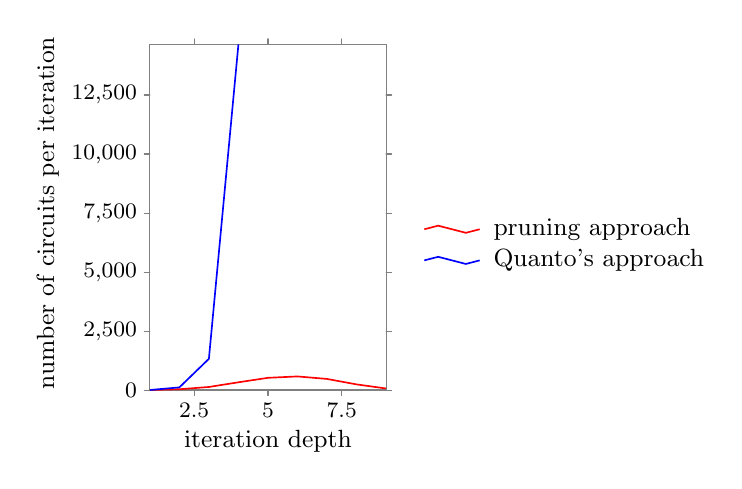
\begin{tikzpicture}[]
    \datavisualization [
      scientific axes,
          x axis={label={iteration depth}, attribute=depth, length=3cm, ticks=few},
         y axis={label={number of circuits per iteration}, attribute=circuits, scaling=0 at 0cm and 15000 at 4.5cm},
          visualize as line/.list={quanto, pruned},
      pruned={style=red, label in legend={text={pruning approach}}},
       quanto={style=blue, label in legend={text={Quanto's approach}}}]
    
     data [set=pruned] {
      depth, circuits
      1, 11
      2, 42
      3, 139
      4, 337
      5, 526
      6, 585
      7, 479
      8, 248
      9, 75
    }
    
    data [set=quanto] {
      depth, circuits
      1, 11
      2, 121
      3, 1331
      4, 14641
    };
  \end{tikzpicture}
  \caption{$n = 2$, $gs=[I,H,X,CX]$}
  \label{fig:comp}
\end{figure}
A prototype implementation was developed in Python, using Qiskit and Numpy frameworks. This included both the original Quanto algorithm and the new pruning approach. The optimization part was excluded as it does not significantly differ from the original and would exceed the project scope. The prototype demonstrates the pruning approach's efficiency, reducing the search space and maintaining optimal circuit identities, resulting in a smaller database and faster optimization (Fig. \ref{fig:comp}).

%-------------------------------------------------------------------------------
\bibliographystyle{plain}
\bibliography{report}

%%%%%%%%%%%%%%%%%%%%%%%%%%%%%%%%%%%%%%%%%%%%%%%%%%%%%%%%%%%%%%%%%%%%%%%%%%%%%%%%
\end{document}
%%%%%%%%%%%%%%%%%%%%%%%%%%%%%%%%%%%%%%%%%%%%%%%%%%%%%%%%%%%%%%%%%%%%%%%%%%%%%%%%

%%  LocalWords:  endnotes includegraphics fread ptr nobj noindent
%%  LocalWords:  pdflatex acks
